\documentclass[a4paper,10pt]{article}

\usepackage{appendixnumberbeamer}
\usepackage{booktabs}
\usepackage[scale=2]{ccicons}
\usepackage{pgfplots}
\usepackage{xspace}
\usepackage{bookmark}
\usepackage{amssymb}
\usepackage{mathtools}
\usepackage[normalem]{ulem}
\usepackage[T1]{fontenc}
\usepackage[sfdefault,book]{FiraSans}
\usepackage{FiraMono}
\usepackage{fontawesome}
\usepackage{listings}
\usepackage{hyperref}
\usepackage[10pt]{moresize}

\renewcommand*\familydefault{\ttdefault}

\renewcommand{\thefootnote}{\fnsymbol{footnote}}
\renewcommand{\MintedPygmentize}{/home/thiago/.local/bin/pygmentize}

\definecolor{light-gray}{gray}{0.95}
\renewcommand\lstlistingname{Código}
\DeclareCaptionFormat{listing} {
  \parbox{\textwidth}{\hspace{-0.2cm}#1#2#3}
}
\DeclareCaptionFont{black}{\color{black}}
\captionsetup[lstlisting]{
  format=listing,
  labelfont=black,
  textfont=black,
  singlelinecheck=true,
  margin=0pt,
  font={tt,footnotesize,bf}
}

\lstset{
  basicstyle=\footnotesize\ttfamily,
  escapeinside={\%*}{*)},
  mathescape=true,
  showspaces=false,
  showtabs=false,
  showstringspaces=false,%
  % backgroundcolor=\color{light-gray},
  rulesepcolor=\color{black},
  frame=shadowbox,
  literate=
  {á}{{\'a}}1 {é}{{\'e}}1 {í}{{\'i}}1 {ó}{{\'o}}1 {ú}{{\'u}}1
  {Á}{{\'A}}1 {É}{{\'E}}1 {Í}{{\'I}}1 {Ó}{{\'O}}1 {Ú}{{\'U}}1
  {à}{{\`a}}1 {è}{{\`e}}1 {ì}{{\`i}}1 {ò}{{\`o}}1 {ù}{{\`u}}1
  {À}{{\`A}}1 {È}{{\'E}}1 {Ì}{{\`I}}1 {Ò}{{\`O}}1 {Ù}{{\`U}}1
  {ä}{{\"a}}1 {ë}{{\"e}}1 {ï}{{\"i}}1 {ö}{{\"o}}1 {ü}{{\"u}}1
  {Ä}{{\"A}}1 {Ë}{{\"E}}1 {Ï}{{\"I}}1 {Ö}{{\"O}}1 {Ü}{{\"U}}1
  {â}{{\^a}}1 {ê}{{\^e}}1 {î}{{\^i}}1 {ô}{{\^o}}1 {û}{{\^u}}1
  {Â}{{\^A}}1 {Ê}{{\^E}}1 {Î}{{\^I}}1 {Ô}{{\^O}}1 {Û}{{\^U}}1
  {Ã}{{\~A}}1 {ã}{{\~a}}1 {Õ}{{\~O}}1 {õ}{{\~o}}1
  {œ}{{\oe}}1 {Œ}{{\OE}}1 {æ}{{\ae}}1 {Æ}{{\AE}}1 {ß}{{\ss}}1
  {ű}{{\H{u}}}1 {Ű}{{\H{U}}}1 {ő}{{\H{o}}}1 {Ő}{{\H{O}}}1
  {ç}{{\c c}}1 {Ç}{{\c C}}1 {ø}{{\o}}1 {å}{{\r a}}1 {Å}{{\r A}}1
  {€}{{\euro}}1 {£}{{\pounds}}1 {«}{{\guillemotleft}}1
  {»}{{\guillemotright}}1 {ñ}{{\~n}}1 {Ñ}{{\~N}}1 {¿}{{?`}}1
}

\setminted{
  fontsize=\footnotesize,
  style=xcode,
  frame=single,
  framesep=3\fboxsep,
  labelposition=topline,
}


\title{Exercícios 02 (Grafos)}
\posttitle{\end{center}}

\begin{document}

\maketitle

\emergencystretch 3em

{\raggedright \textbf{Para todas as questões, assuma que as listas de adjacência estão ordenadas por ordem crescente alfabética/numérica}.}

\bigskip

\begin{multicols*}{2}
\setlength{\leftmargini}{0pt}
\begin{enumerate}
  % SKIENA, S. S. The Algorithm Design Manual, 2nd Edition -- 5.31
  \item Quais são as estruturas de dados utilizadas na BFS e na DFS? % Pilha e fila, respectivamente

  %%%%%%%%%%%%%%%%%%%%%%%%%%%%%%%%%%%%%%%%%%%%%%%%
  % BFS                                          %
  %%%%%%%%%%%%%%%%%%%%%%%%%%%%%%%%%%%%%%%%%%%%%%%%
  % CORMEN, T. H.; LEISERSON, C. E.; RIVEST, R. L.; STEIN, C. Introduction to Algorithms, 3rd Edition -- 22.2-1
  \item Obtenha os valores de distância e parentesco para a execução da BFS no grafo dirigido a seguir, usando o vértice 3 como inicial.
  % (1/0) (2/3)    (3/0)
  %       /        /  |
  %      /        /   |
  %     /        /    |
  % (4/2)-----(5/1) (6/1)
  %
  %  1  2  3  4  5  6
  % -1  4 -1  5  3  3

  \begin{center}
    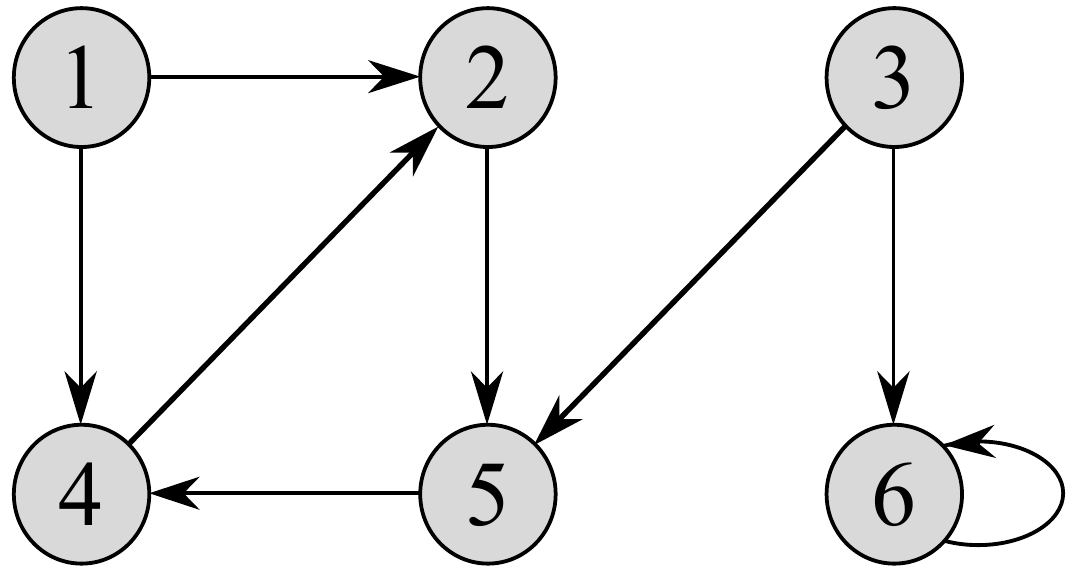
\includegraphics[width=.8\linewidth]{graph2.png}
  \end{center}

  % CORMEN, T. H.; LEISERSON, C. E.; RIVEST, R. L.; STEIN, C. Introduction to Algorithms, 3rd Edition -- 22.2-2
  \item Obtenha os valores de distância e parentesco para a execução da BFS no grafo não-dirigido a seguir, usando o vértice u como inicial.
  %
  % (r/4)--(s/3)  (t/1)--(u/0)
  %   |      |    /      / |
  %   |      |   /      /  |
  %   |      |  /      /   |
  % (v/5)  (w/2)  (x/1)  (y/1)
  %
  %  r  s  t  u  v  w  x  y
  %  s  w  u -1  r  t  u  u

  \begin{center}
    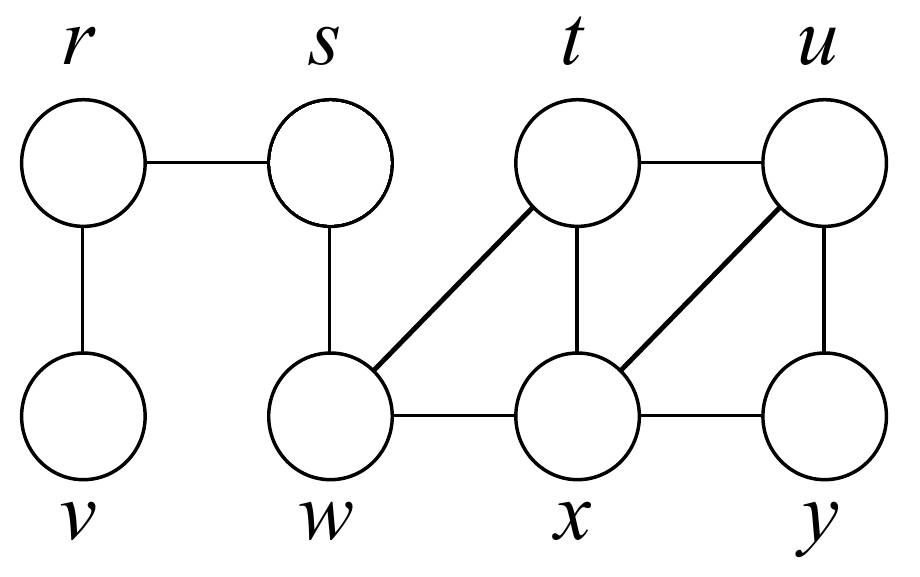
\includegraphics[width=\linewidth]{graph3.png}
  \end{center}

  % CORMEN, T. H.; LEISERSON, C. E.; RIVEST, R. L.; STEIN, C. Introduction to Algorithms, 3rd Edition -- 22.2-5
  \item Usando a figura da questão anterior, mostre como diferenças na ordem interna de cada lista de adjacência podem alterar a árvore de parentesco gerada pela BFS.

  %%%%%%%%%%%%%%%%%%%%%%%%%%%%%%%%%%%%%%%%%%%%%%%%
  % DFS                                          %
  %%%%%%%%%%%%%%%%%%%%%%%%%%%%%%%%%%%%%%%%%%%%%%%%
  % CORMEN, T. H.; LEISERSON, C. E.; RIVEST, R. L.; STEIN, C. Introduction to Algorithms, 3rd Edition -- Figure 22.5
  \item Obtenha os valores de tempo e parentesco e as classificações das arestas para a execução da DFS no grafos dirigidos a seguir. Use o vértice s como inicial para o primeiro grafo e assuma que os vértices são processados em ordem alfabética no segundo grafo.
  % PRIMEIRO GRAFO
  %
  % Arestas
  % s - w Árvore
  % s - z Direta
  % t - u Árvore
  % t - v Direta
  % u - t Retorno
  % u - v Árvore
  % v - s Cruzada
  % v - w Cruzada
  % w - x Árvore
  % x - z Árvore
  % y - x Retorno
  % z - w Retorno
  % z - y Árvore
  %
  %    |   s   t   u   v   w   x   y   z
  % ---|--------------------------------
  % P  |  -1  -1   t   u   s   w   z   x
  % Ti |   1  11  12  13   2   3   5   4
  % To |  10  16  15  14   9   8   6   7
  %
  % (s (w (x (z (y y) z) x) w) s) (t (u (v v) u) t)
  %
  % SEGUNDO GRAFO
  %
  % Arestas
  % q - s Árvore
  % q - t Árvore
  % q - w Direta
  % r - u Árvore
  % r - y Cruzada
  % s - v Árvore
  % t - y Árvore
  % t - x Árvore
  % u - y Cruzada
  % v - w Árvore
  % w - s Retorno
  % x - z Árvore
  % y - q Retorno
  % z - x Retorno
  %
  %    |   q   r   s   t   u   v   w   x   y   z
  % ---|----------------------------------------
  % P  |  -1  -1   q   q   r   s   v   t   t   x
  % Ti |   1  17   2   8  18   3   4   9  13  10
  % To |  16  20   7  15  19   6   5  12  14  11
  %
  % (q (s (v (w  w) v) s) (t (x (z z) x) (y y) t) q) (r (u u) r)

  \begin{center}
    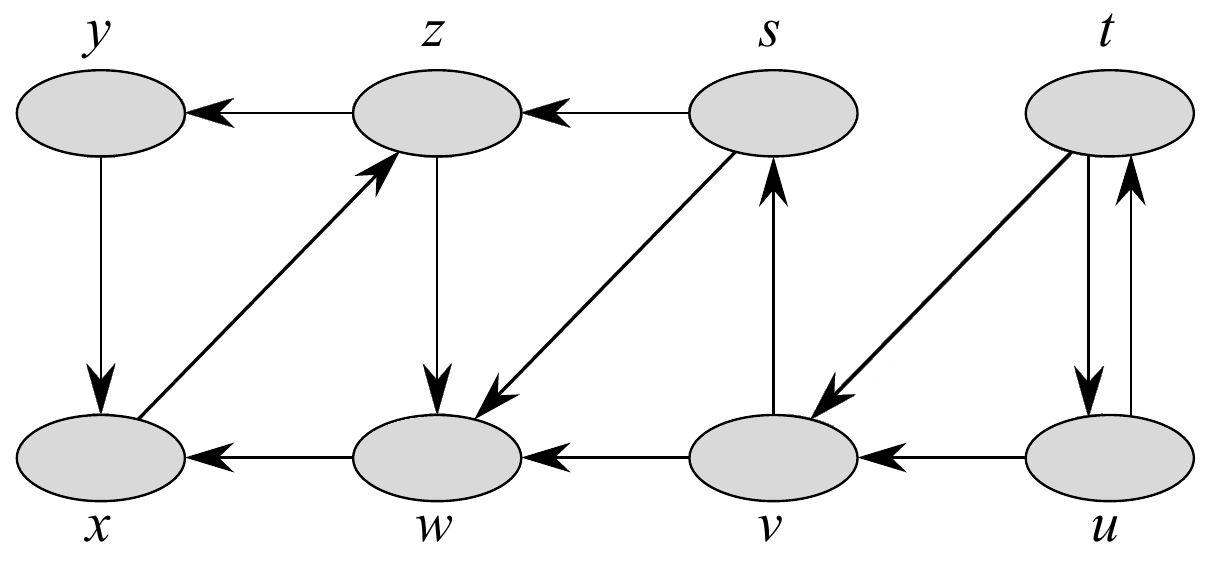
\includegraphics[width=\linewidth]{graph4.png}
  \end{center}

  \begin{center}
    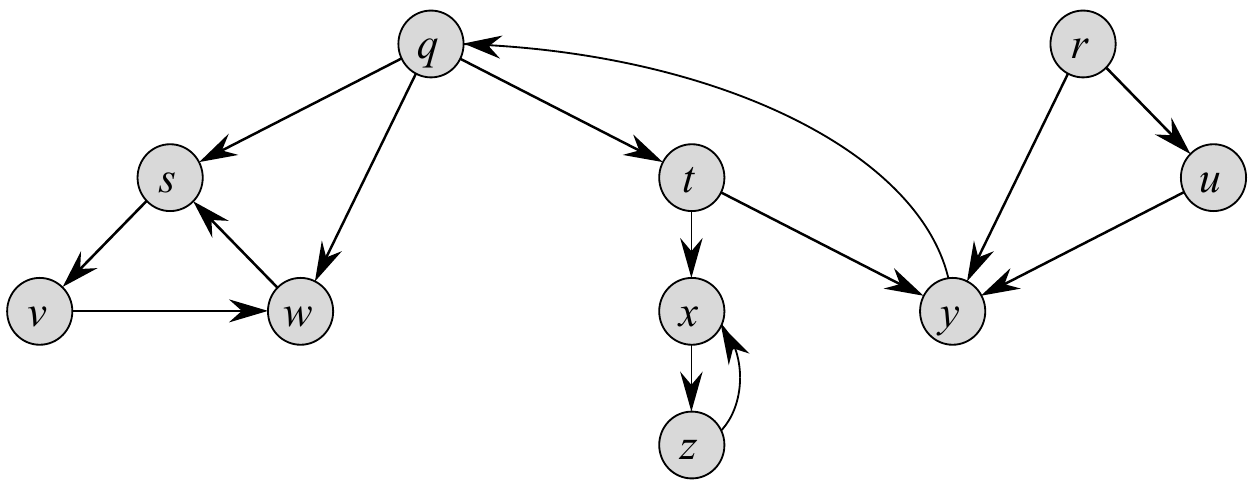
\includegraphics[width=\linewidth]{graph5.png}
  \end{center}

  % CORMEN, T. H.; LEISERSON, C. E.; RIVEST, R. L.; STEIN, C. Introduction to Algorithms, 3rd Edition -- 22.3-3
  \item \xout{Mostre a estrutura de parênteses gerada pela DFS para o grafo da questão 2, começando a partir do vértice 1.}
  % ARESTAS
  % 1 - 2 Árvore
  % 1 - 4 Direta
  % 2 - 5 Árvore
  % 3 - 5 Cruzada
  % 3 - 6 Árvore
  % 4 - 2 Retorno
  % 5 - 4 Árvore
  % 6 - 6 Cruzada
  %
  %    |   1   2   3   4   5   6
  % ---|------------------------
  % P  |  -1   1  -1   5   2   3
  % Ti |   1   2   9   4   3  10
  % To |   8   7  12   5   6  11
  %
  % (1 (2 (5 (4 4) 5) 2) 1) (3 (6 6) 3)

  %%%%%%%%%%%%%%%%%%%%%%%%%%%%%%%%%%%%%%%%%%%%%%%%
  % ORDENAÇÃO TOPOLÓGICA                         %
  %%%%%%%%%%%%%%%%%%%%%%%%%%%%%%%%%%%%%%%%%%%%%%%%
  \item Faça uma ordenação topológica para cada grafo a seguir
  \bigskip

  % SKIENA, S. S. The Algorithm Design Manual, 2nd Edition -- 5.2
  \begin{center}
    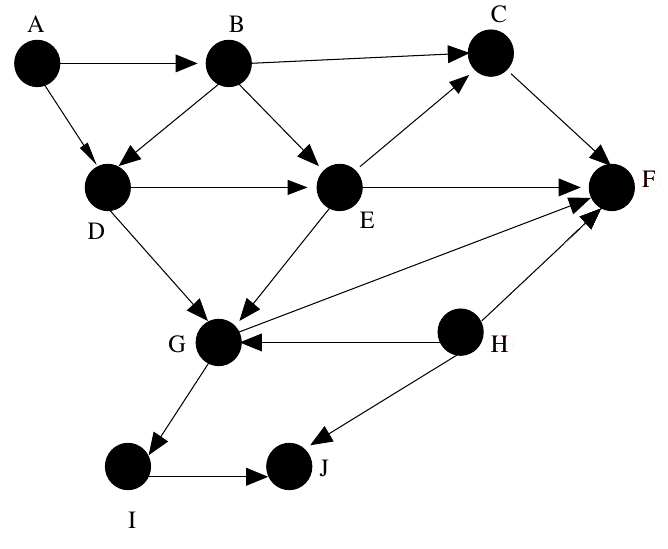
\includegraphics[width=\linewidth]{graph1.png}
  \end{center}
  % H A B D E G I J C F

  % CORMEN, T. H.; LEISERSON, C. E.; RIVEST, R. L.; STEIN, C. Introduction to Algorithms, 3rd Edition -- 22.4-1
  \begin{center}
    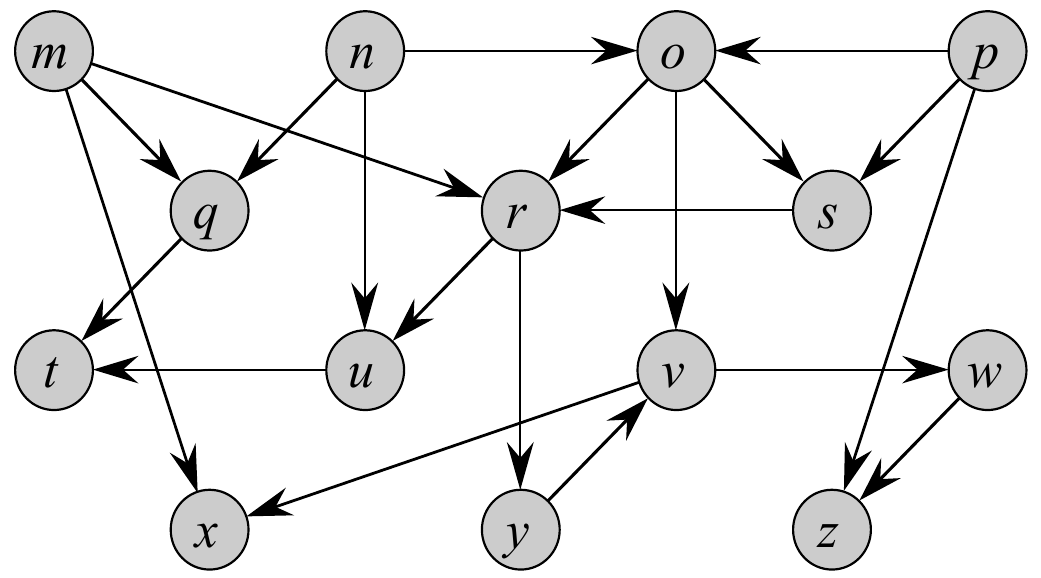
\includegraphics[width=\linewidth]{graph6.png}
  \end{center}
  % p n o s m r y v x w z u q t

  %%%%%%%%%%%%%%%%%%%%%%%%%%%%%%%%%%%%%%%%%%%%%%%%
  % COMPONENTES FORTEMENTE CONECTADOS            %
  %%%%%%%%%%%%%%%%%%%%%%%%%%%%%%%%%%%%%%%%%%%%%%%%
  % CORMEN, T. H.; LEISERSON, C. E.; RIVEST, R. L.; STEIN, C. Introduction to Algorithms, 3rd Edition -- 22.5-2
  \item Identifique os componentes fortemente conectados no segundo grafo da questão 5 e mostre o grafo acíclico resultante.
  %    qty----r
  %   / | \  |
  % svw |  \ |
  %     xz   u
\end{enumerate}
\end{multicols*}
\end{document}
